\chapter{\IfLanguageName{dutch}{Stand van zaken}{State of the art}}%
\label{ch:stand-van-zaken}

% Tip: Begin elk hoofdstuk met een paragraaf inleiding die beschrijft hoe
% dit hoofdstuk past binnen het geheel van de bachelorproef. Geef in het
% bijzonder aan wat de link is met het vorige en volgende hoofdstuk.

% Pas na deze inleidende paragraaf komt de eerste sectiehoofding.

\section{Network and Information Security 2}%
\label{sec:nis2}

\section{Huidige aanpak van asset management}%
\label{sec:huidige_aanpak_van_asset_management}

\subsection{Infrastructure as Code}%
\label{sub:iac}

Sinds de opkomst van computernetwerken is het uitrollen en beheren van servers en netwerken altijd een uitdagende taak geweest.
Infrastructure as Code (IaC) is een concept dat de laatste jaren steeds meer aan populariteit wint. Dit komt vooral doordat het beheerders van zulke netwerken in staat stelt om hun configuratie en infrastructuur vast te leggen in code, in plaats van handmatig te configureren.
Binnen deze code kunnen veelvoorkomende, complexe taken automatisch worden uitgevoerd, en dit alles op een geteste en foutloze manier~\autocite{chef-what-is-iac}.

IaC is gebaseerd op drie fundamentele concepten~\autocite{chef-what-is-iac}:
\begin{itemize}
    \item Automatisering: Het aanpassen van handmatige configuratie en het uitrollen van nieuwe servers worden allemaal geautomatiseerd met behulp van code.
    \item Testen: IT, DevOps en SecOps processen kunnen met vertrouwen worden uitgevoerd omdat de code getest is.
    \item Idempotentie: Processen worden niet alleen toegepast op nieuwe servers, maar ook op bestaande servers om een consistente configuratie te behouden.
\end{itemize}

E\'en van de grootste voordelen van Iac is de verhoging van de effici\"entie~\autocite{splunk-benefits-iac}.
Doordat veel taken geautomatiseerd worden, kunnen beheerders zich richten op andere, meer complexe taken.
Zo heeft Red Hat in 2016 een casestudy gepubliceerd~\autocite{case-study-nasa-iac} waarin ze NASA's resultaten van hun overstap naar de IaC-tools Ansible en Ansible Tower hebben geanalyseerd.
Hierin geven ze aan dat het updateproces van nasa.gov van meer dan 1 uur is teruggebracht tot minder dan 5 minuten.
Het langdurige proces van het patchen van updates werd teruggebracht van een proces dat meerdere dagen in beslag nam naar een proces van ongeveer 45 minuten.

Het Duitse Federaal Ministerie van Voedsel en Landbouw (Bundesanstalt f\"ur Landwirtschaft und Ern\"ahrung, of BLE), heeft ook bepaalde IT-toepassingen met 50\% kunnen versnellen dankzij een overstap naar een IaC-aanpak~\autocite{case-study-ble-iac}.
In de studie bespreken ze kort waarom ze hebben besloten over te schakelen naar een IaC-aanpak en geven ze een paar voorbeelden van hoe ze voorheen te werk gingen en hoe ze dit met IaC hebben aangepakt.
Tijdens de implementatie hebben ze 1.000 virtuele machines overgeschakeld van Debian en SUSE Linux naar Red Hat Enterprise Linux, ook bekend als RHEL.
Deze machines worden beheerd met behulp van Satellite en geautomatiseerd met Ansible.

Condition assessments is één van de belangrijkste componenten van IT asset management (IAM)~\autocite{ibm-what-is-iam}.
Dit proces houdt in dat men op elk moment de huidige staat kan bekijken van een asset.
Doordat IaC de configuratie van een asset vastlegt in code en zorgt dat deze consistent is, kan IaC ondersteuning bieden bij dit proces.

\subsection{Data Center Infrastructure Management}
\label{sub:dcim}

\subsection{IP Address Management}
\label{sub:ipam}

\subsection{Snipe-IT}
\label{sub:snipe-it}

Snip-IT is een open-source webapplicatie ontwikkeld door Grokability sinds 2013~\autocite{snipe-it-introduction}, die gericht is op IT-assetmanagement.
Het idee achter Snipe-IT komt voort uit de vroegere aanpak van het bedrijf, toen het voornamelijk nog gebruik maakte van spreadsheets om hun bedrijfsmiddelen te inventariseren.
Het doel was om een applicatie te ontwikkelen die deze taak op een meer georganiseerde en effici\"ente manier kon uitvoeren.

\begin{figure}[h!]
    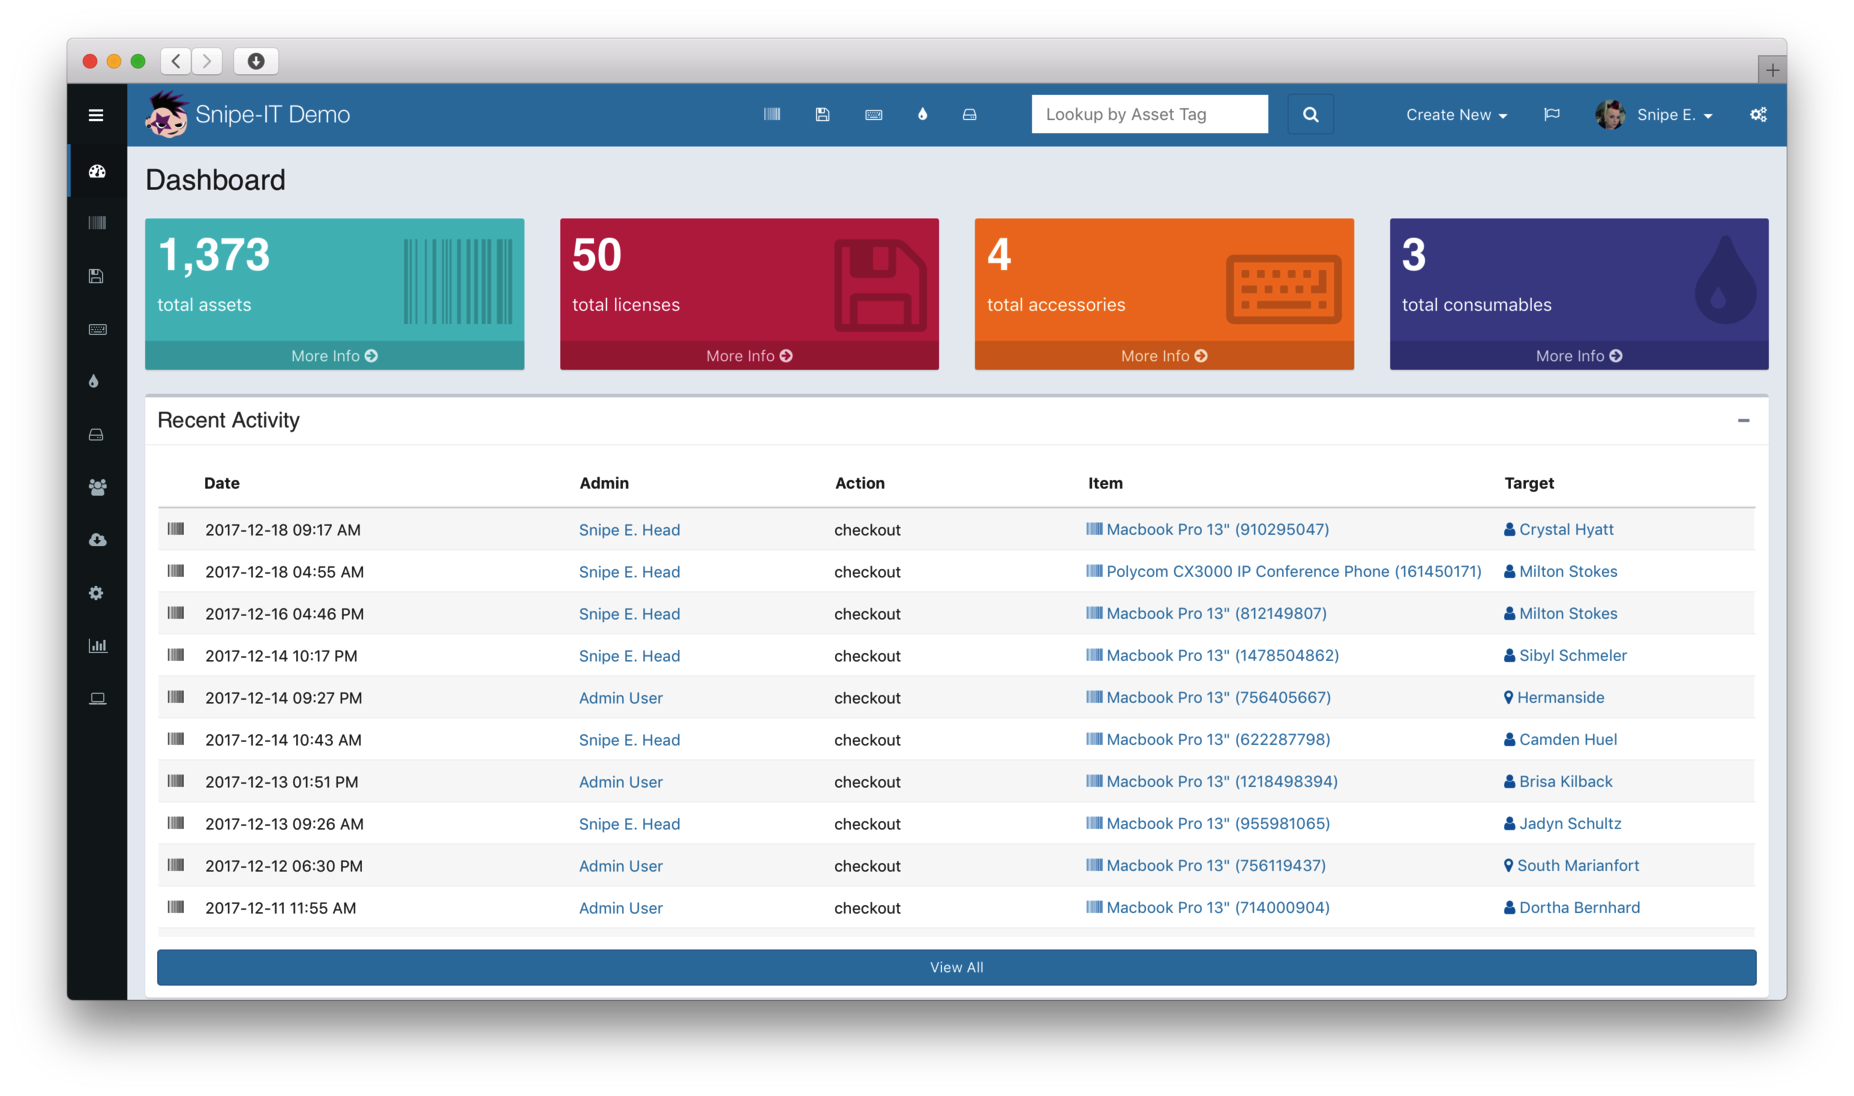
\includegraphics[width=\textwidth]
    {./graphics/snipe-dashboard.png}
    \caption{\label{fig:snipe-it-dashboard}Snip-IT dashboard.}
\end{figure}

De software biedt een gebruiksvriendelijke webinterface (\ref{fig:snipe-it-dashboard}) waarmee bedrijfsmiddelen, licenties, garanties en meer gemakkelijk kunnen worden beheerd.
Wanneer men kiest voor de self-hosted optie is de software gratis beschikbaar, terwijl ook verschillende cloud-gebaseerde optie beschikbaar zijn tegen een jaarlijkse bijdrage.
Deze prijs varieert afhankelijk van de nodige features en support.
Alle code en services gerelateerd aan Snipe-IT zijn vrij beschikbaar op GitHub~\autocite{snipe-it-github}.

Enkele van de belangrijkste functies van Snipe-IT zijn~\autocite{snipe-it-features}, maar zijn niet beperkt tot:
\begin{itemize}
    \item Gemakkelijk zien welke assets zijn toegewezen, aan wie, en hun fysieke locatie
    \item In één klik inchecken
    \item Assetmodellen waarmee je gemeenschappelijke functies kunt groeperen
    \item Vereisen van Gebruikersacceptatie (Eindgebruikers EULA's/Gebruiksvoorwaarden) bij Uitchecken
    \item E-mailmeldingen voor het verlopen van garanties en licenties
    \item Integratie met de meeste handheld barcode scanners en QR-codelezer apps
    \item Snelle en eenvoudige asset-audit
    \item Voeg je eigen aangepaste velden toe voor extra assetattributen
    \item Assets gemakkelijk importeren en exporteren
    \item Genereer QR-code labels voor eenvoudige mobiele toegang en labeling
    \item Assets gemarkeerd als aanvraagbaar kunnen worden aangevraagd door een gebruiker
    \item Assets behouden een volledige geschiedenis inclusief uitchecken, inchecken en onderhoud
    \item Optionele digitale handtekeningen bij assetacceptatie
\end{itemize}

\subsection{Nagios}
\label{sub:nagios}

\subsection{Lansweeper}
\label{sub:lansweeper}

Lansweeper, opgericht in 2004, is een Belgisch commercieel IT discovery \& inventory platform~\autocite{lansweeper-history}.
Het is een veelgebruikte tool voor het scannen, bijhouden en beheren van IT-assets binnen een organisatie.
Met functionaliteiten voor zowel hardware- als software-inventarisatie, biedt Lansweeper gebruikers een uitgebreid overzicht van alle IT-assets in hun netwerk.

Het grote voordeel van Lansweeper ten opzichte van andere tools, zoals Snipe-IT, is dat het een volledig geautomatiseerde oplossing biedt~\autocite{lansweeper-features}.
Dit betekent dat het platform in staat is om automatisch alle IT-assets binnen een netwerk te detecteren, zonder handmatige configuratie of de noodzaak om op elk systeem een agent te installeren~\autocite{lansweeper-getting-started}.
Dit gebeurt met behulp van verschillende protocollen, waaronder SNMP.
De gedetecteerde informatie wordt vervolgens opgeslagen in een centrale database en is toegankelijk via een gebruiksvriendelijke webinterface.

\begin{figure}[h!]
    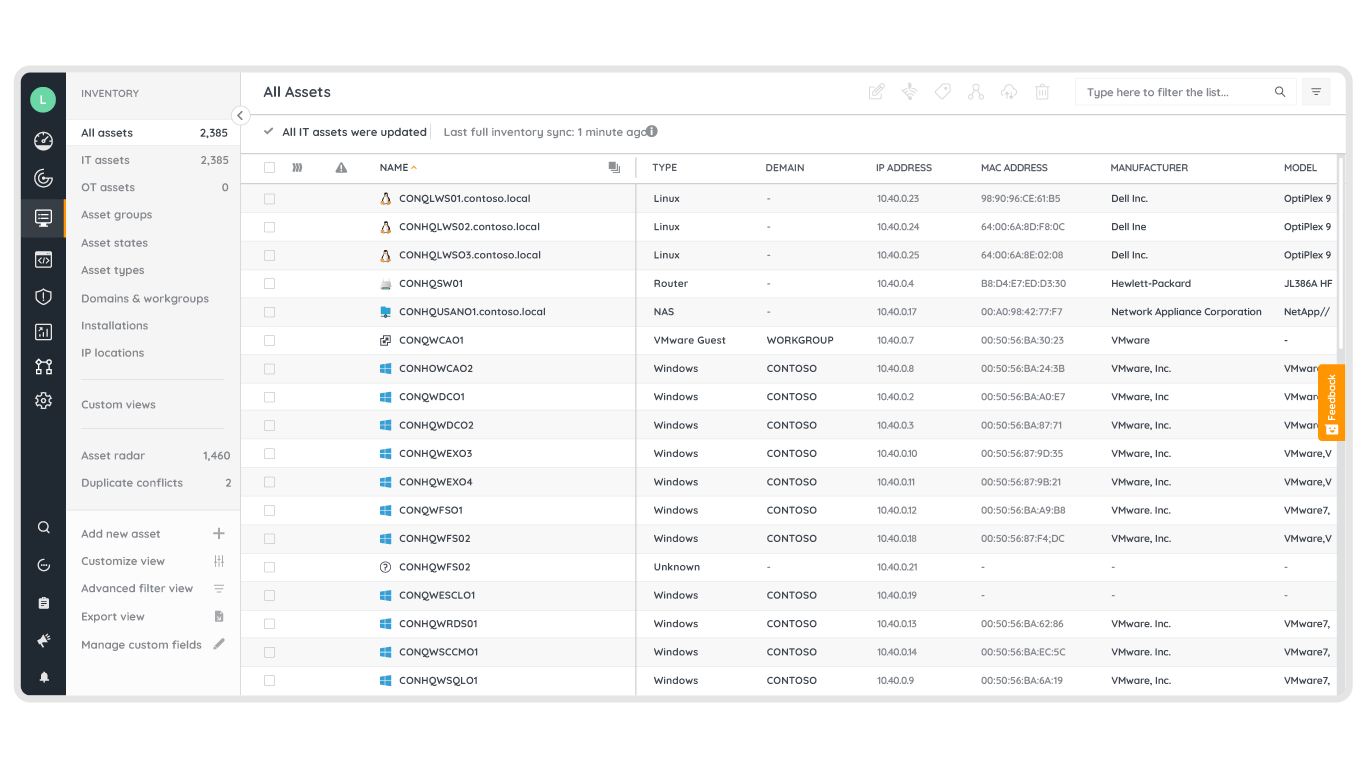
\includegraphics[width=\textwidth]
    {./graphics/lansweeper-dashboard.png}
    \caption{\label{fig:lansweeper-dashboard}Lansweeper dashboard.}
\end{figure}

Gebruikers kunnen aangepaste rapporten genereren over verschillende aspecten van hun IT-infrastructuur, zoals hardwareconfiguraties, softwarelicenties, patchniveaus en meer.
Deze rapporten zijn bruikbaar voor audits, nalevingscontroles en capaciteitsplanning.
